
%(BEGIN_QUESTION)
% Copyright 2007, Tony R. Kuphaldt, released under the Creative Commons Attribution License (v 1.0)
% This means you may do almost anything with this work of mine, so long as you give me proper credit

The lever transmitter (LT) in this level control system is hydrostatic; i.e. it senses liquid level in the vessel based on the hydrostatic pressure exerted by the liquid's height in the vessel:

$$\includegraphics[width=15.5cm]{i02960x01.eps}$$

Suppose the density of the liquid within the vessel decreases.  What effect will this have on the controlled liquid level?  In other words, what will the liquid level inside the vessel do over time in response to this change in density?  Be sure to explain {\it why} the level will be affected (or not affected), not just what will happen to the level.

\vfil 

\underbar{file i02960}
\eject
%(END_QUESTION)





%(BEGIN_ANSWER)

This is a graded question -- no answers or hints given!

%(END_ANSWER)





%(BEGIN_NOTES)

The operating principle of a hydrostatic liquid level sensor is that the pressure sensed by the device is proportional to the product of liquid density and vertical liquid column height ($P = \gamma h$).  We may reliably infer liquid level with this type of instrument only if the liquid's density is known and constant.  

\vskip 10pt

Here we are told that the liquid density is not constant, but rather decreases.  This will cause the hydrostatic pressure to decrease even if the liquid level remains the same, thus ``fooling'' the transmitter into thinking liquid level has decreased.

\vskip 10pt

If the transmitter ``thinks'' there is less liquid level than there actually is, the controller will sense this apparent decrease in level and will act to {\it raise} the liquid level back to the proper setpoint, resulting in an actual liquid level exceeding setpoint.  The controller's indication of liquid level, however, will remain equal to setpoint, thereby hiding the problem from operators' views.

%INDEX% Basics, control loop troubleshooting: determining effect of specified fault(s)

%(END_NOTES)


